\documentclass[10.5pt]{article}
\usepackage{amsmath,amssymb,amsthm}
\usepackage{listings}
\usepackage{graphicx}
\usepackage[shortlabels]{enumitem}
\usepackage{tikz}
\usepackage[margin=1in]{geometry}
\usepackage{fancyhdr}
\usepackage{epsfig} %% for loading postscript figures
\usepackage{amsmath}
\usepackage{float}
\usepackage{amssymb}
\usepackage{caption}
\usepackage{subfigure}
\usepackage{graphics}
\usepackage{titlesec}
\usepackage{mathrsfs}
\usepackage{amsfonts}
\usepackage{indentfirst}
\usepackage{fancybox}
\usepackage{tikz}
\usepackage{algorithm}
\usepackage{algcompatible}
% \usepackage{fontspec}

\renewcommand{\baselinestretch}{1.2}%Adjust Line Spacing
%\geometry{left=2.0cm,right=2.0cm,top=2.0cm,bottom=2.0cm}% Adjust Margins of the File
\usepackage{tikz-qtree}
\usetikzlibrary{graphs}
\tikzset{every tree node/.style={minimum width=2em,draw,circle},
	blank/.style={draw=none},
	edge from parent/.style=
	{draw,edge from parent path={(\tikzparentnode) -- (\tikzchildnode)}},
	level distance=1.2cm}
\setlength{\parindent}{0pt}
%\setlength{\parskip}{5pt plus 1pt}
\setlength{\headheight}{13.6pt}
\newcommand\question[2]{\vspace{.25in}\hrule\textbf{#1: #2}\vspace{.5em}\hrule\vspace{.10in}}
\renewcommand\part[1]{\vspace{.10in}\textbf{(#1)}}
%\newcommand\algorithm{\vspace{.10in}\textbf{Algorithm: }}
\newcommand\correctness{\vspace{.10in}\textbf{Correctness: }}
\newcommand\runtime{\vspace{.10in}\textbf{Running time: }}
\pagestyle{fancyplain}
% Create horizontal rule command with an argument of height
\newcommand{\horrule}[1]{\rule{\linewidth}{#1}}
% Set the title here
\title{
	\normalfont \normalsize
	\textsc{ShanghaiTech University} \\ [25pt]
	\horrule{0.5pt} \\[0.4cm] % Thin top horizontal rule
	\huge CS101 Algorithms and Data Structures\\ % The assignment title
	\LARGE Fall 2020\\
	\LARGE Homework 7\\
	\horrule{2pt} \\[0.5cm] % Thick bottom horizontal rule
}
% wrong usage of \author, never mind
\author{}
\date{Due date: 23:59, November 2, 2020}

% set the header and footer
\pagestyle{fancy}
\lhead{CS101 Algorithms and Data Structures}
\chead{Homework 7}
\rhead{Due date: 23:59, November 2, 2020}
\cfoot{\thepage}
\renewcommand{\headrulewidth}{0.4pt}
\newtheorem{Q}{Question}
% special settings for the first page
\fancypagestyle{firstpage}
{
	\renewcommand{\headrulewidth}{0pt}
	\fancyhf{}
	\fancyfoot[C]{\thepage}
}

% Add the support for auto numbering
% use \problem{title} or \problem[number]{title} to add a new problem
% also \subproblem is supported, just use it like \subsection
\newcounter{ProblemCounter}
\newcounter{oldvalue}
\newcommand{\problem}[2][-1]{
	\setcounter{oldvalue}{\value{secnumdepth}}
	\setcounter{secnumdepth}{0}
	\ifnum#1>-1
	\setcounter{ProblemCounter}{0}
	\else
	\stepcounter{ProblemCounter}
	\fi
	\section{Problem \arabic{ProblemCounter}: #2}
	\setcounter{secnumdepth}{\value{oldvalue}}
}
\newcommand{\subproblem}[1]{
	\setcounter{oldvalue}{\value{section}}
	\setcounter{section}{\value{ProblemCounter}}
	\subsection{#1}
	\setcounter{section}{\value{oldvalue}}
}

% \setmonofont{Consolas}
\definecolor{blve}{rgb}{0.3372549 , 0.61176471, 0.83921569}
\definecolor{gr33n}{rgb}{0.29019608, 0.7372549 , 0.64705882}
\makeatletter
\lst@InstallKeywords k{class}{classstyle}\slshape{classstyle}{}ld
\makeatother
\lstset{language=C++,
	basicstyle=\ttfamily,
	keywordstyle=\color{blve}\ttfamily,
	stringstyle=\color{red}\ttfamily,
	commentstyle=\color{green}\ttfamily,
	morecomment=[l][\color{magenta}]{\#},
	classstyle = \bfseries\color{gr33n}, 
	tabsize=4
}

\begin{document}
	\maketitle
	\thispagestyle{firstpage}
	%\newpage
	\vspace{3ex}
	
	\begin{enumerate}
		\item Please write your solutions in English. 
		
		\item Submit your solutions to gradescope.com.  
		
		\item Set your Full Name to your Chinese name and your STUDENT ID correctly in Account Settings. 
		
		\item If you want to submit a handwritten version, scan it clearly. Camscanner is recommended. 
		
		\item When submitting, match your solutions to the according problem numbers correctly. 
		
		\item No late submission will be accepted.
		
		\item Violations to any of above may result in zero score. 
	\end{enumerate}
	\newpage
	
	%---------------------------------------------------------
\question{1}{(4*2') Multiple Choices}

Each question has one or more correct answer(s). Select all the correct answer(s). For each question, you get $0$ point if you select one or more wrong answers, but you get $1$ point if you select a non-empty subset of the correct answers.\\
\textit{Note that you should write you answers of section 1 in the table below.}
\begin{table}[htbp]
	\begin{tabular}{|p{2cm}|p{2cm}|p{2cm}|p{2cm}|}
		\hline 
		Question 1 & Question 2 & Question 3 & Question 4  \\ 
		\hline 
		&  &  &  \\ 
		\hline 
	\end{tabular} 
\end{table}

\begin{Q}
	Which of the followings are true? 
	\begin{enumerate}[(A)]
		\item For a min-heap, in-order traversal gives the elements in ascending order.
		\item For a min-heap, pre-order traversal gives the elements in ascending order.
		\item For a BST, in-order traversal gives the elements in ascending order.
		\item For a BST, pre-order traversal gives the elements in ascending order.
	\end{enumerate}
\end{Q}

\begin{Q}
    Which of the following statements are true for an AVL-tree?
	\begin{enumerate}[(A)]
		\item Inserting an item can unbalance non-consecutive nodes on the path from the root to the inserted item before the restructuring.
		\item Inserting an item can cause at most one node imbalanced before the restructuring.
		\item Removing an item in leaf nodes can cause at most one node imbalanced before the restructuring.
		\item Only at most one node-restructuring has to be performed after inserting an item.
	\end{enumerate}
\end{Q}

\begin{Q}
	Consider an AVL tree whose height is h, which of the following are true?
	\begin{enumerate}[(A)]
		\item This tree contains $\Omega(\alpha^h)$ nodes, where $\alpha = \dfrac{1+\sqrt{5}}{2}$.
		\item This tree contains $\Theta(2^h)$ nodes.
		\item This tree contains $O(h)$ nodes in the worst case.
		\item None of the above.
	\end{enumerate}
\end{Q}


\begin{Q}
Which of the following is TRUE?
    \begin{enumerate}
        \item[(A)] The cost of searching an AVL tree is $O(\log n)$ but that of a binary search tree is $O(n)$
        \item[(B)] The cost of searching an AVL tree is $O(\log n)$ but that of a complete binary tree is $O(n \log n)$
        \item[(C)] The cost of searching a binary search tree with height h is $O(h)$ but that of an AVL tree is $O(\log n)$
        \item[(D)] The cost of searching an AVL tree is $O(n log n)$ but that of a binary search tree is $O(n)$
    \end{enumerate}
\end{Q}

\newpage
	%---------------------------------------------------------
\question{2}{(3'+5'+8') BST and AVL Tree}

\begin{Q}
Draw a valid BST of minimum height containing the keys 1, 2, 3, 5, 7, 8, 9.
\\
\\
\\
\\
\\
\\
\\
\\
\\
\\
\\
\\
\\
\\

\end{Q}

\begin{Q}
Show that for $\forall N > 0$, a complete BST containing N items (without duplicates) is unique. By unique we mean
the BST is the only complete BST that contains exactly those N items. By complete we mean every level of the tree, except possibly the last, is completely filled, and all nodes are as far left as possible. 
\\ 
\textbf{Hint}: Try to prove by contradiction.

\end{Q}

\newpage
\begin{Q}BST and AVL Tree

\begin{enumerate}[(1)]
    \item 
        Given an empty Binary Search Tree, insert the sequence of integers $15, 20, 23, 10, 13, 7, 30, 25$ from left to right into the BST. Draw the final BST.\\
        
        \vspace{30ex}
        
    \item
        Replace the BST in the question (1) with an AVL tree and insert the same sequence of integers into it. Draw the final AVL tree.\\
        \vspace{30ex}
    \item
        For the final AVL tree in the question (2), delete $7$. Draw the AVL tree after deletion.\\
        \vspace{30ex}
\end{enumerate}


\end{Q}

\pagebreak

\question{3}{Magic BST (6')}
Consider the binary search tree below. Each symbol represents an object stored in the BST. \\
\begin{minipage}{1\textwidth}
	\centering
	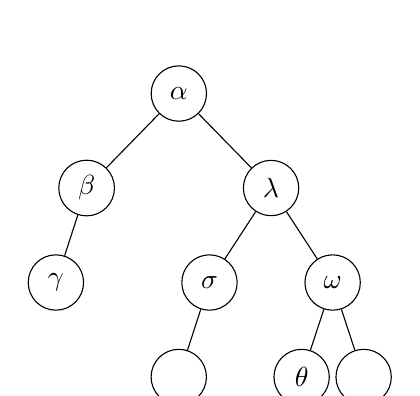
\begin{tikzpicture}
	\Tree
	[.$\alpha$
		[.$\beta$
			\edge[];[.$\gamma$
			]
			\edge[blank]; \node[blank]{};
		]
		[.$\lambda$
			\edge[];[.$\sigma$
			\edge[];\node[]{};
			\edge[blank]; \node[blank]{};
			]
			\edge[];[.$\omega$
			\edge[];[.$\theta$
			]
			\edge[];\node[]{};
			]
		]
	]
	\end{tikzpicture}
\end{minipage} \\
\begin{Q} (3') Based on the ordering given by the tree above, fill in the BST below with valid symbols. Symbols
must be unique. You may only use the 7 printed symbols (do not include any symbols from part b).
\begin{minipage}{1\textwidth}
	\centering
	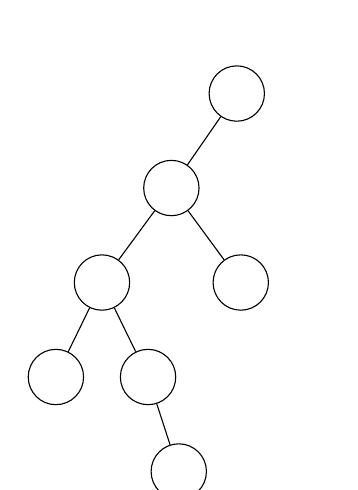
\begin{tikzpicture}
	\Tree
	[.\node[]{};
		\edge[];[.\node[]{};
		\edge[];[.\node[]{};
		\edge[];[.\node[]{};]
		\edge[];[.\node[]{};
		\edge[blank];[.\node[blank]{};]
		\edge[];[.\node[]{};]
		]
		]
		\edge[];[.\node[]{};]
		]
		\edge[blank]; \node[blank]{};
	]
	\end{tikzpicture}
\end{minipage} \\
\end{Q}

\begin{Q} (3') For each of the insertion operations below, use the information given to "insert" the element into the
\textbf{TOP TREE WITH PRINTED SYMBOLS, NOT THE TREE WITH YOUR HANDWRITTEN 
SYMBOLS} by drawing the object (and any needed links) onto the tree. You can assume the objects are
inserted in the order shown below. You should not change anything about the original tree; you should
only add links and nodes for the new objects. If there is not enough information to determine where the
object should be inserted into the tree, circle “not enough information”. If there is enough information,
circle “drawn in the tree above” and \textbf{draw in the tree AT THE TOP OF THE PAGE.}

\begin{table}[htbp]
	\centering
	\begin{tabular}{cccc}
		insert($\phi$): & $\phi>\omega$ & Draw In Tree Above & Not enough Information \\ 
		insert($\chi$): & $\chi>\gamma$&  Draw In Tree Above & Not enough Information \\
		insert($\xi$): & $\alpha<\xi<\sigma$&  Draw In Tree Above & Not enough Information \\
		insert($\mu$): & $\lambda<\mu<\omega$&  Draw In Tree Above & Not enough Information \\
	\end{tabular} 
\end{table}
\end{Q}

\end{document}